\documentclass[10pt,xcolor=pst,aspectratio=169]{beamer}

\usepackage{etex}

%\usetheme{Boadilla}
%\usecolortheme{wolverine}
\usecolortheme{dolphin}
%\setbeamercovered{transparent}
%\setbeamercolor{block body}{bg=yellow}

\addtobeamertemplate{navigation symbols}{}{%
\usebeamerfont{footline}%
\usebeamercolor[fg]{footline}%
\hspace{1em}%
\insertframenumber/\inserttotalframenumber
}

\usepackage[utf8]{inputenc}
\usepackage[english,russian]{babel}
\usepackage[OT1]{fontenc}
\usepackage{amsmath}
\usepackage{amsfonts}
\usepackage{amssymb}
\usepackage{graphicx}
\usepackage{wrapfig}
\usepackage[3D]{movie15}
\usepackage{animate}
\usepackage{ragged2e}
\usepackage{listings}
\usepackage{color}
\usepackage{pst-all}

\usepackage{tikz}
\usetikzlibrary{
	mindmap,
	arrows, % стрелки
	shapes.misc, % фигуры
	chains, % цепочки
	positioning, % позиционирование элементов
	scopes, % создание дополнительных веток
	shadows % тени
	}

\graphicspath{{pic/}}

\author{\textbf{Губкин А.С.}}

\title[Численные методы в физике]{Численные методы в физике}

\logo{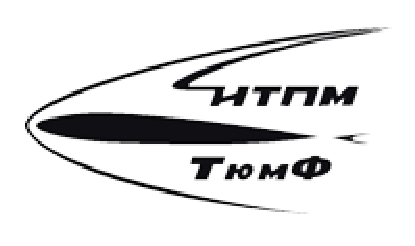
\includegraphics[width=0.1\linewidth]{LOGO_2.EPS}}

\institute[ТюмФ ИТПМ СО РАН]{Тюменский филиал Института теоретической и прикладной механики\\ им. С. А. Христиановича СО РАН, г. Тюмень}

%\date{6 октября 2015 г.}

\begin{document}

\lstset{ %
	language=[ANSI]C++,                 % выбор языка для подсветки (здесь это С++)
	keywordstyle=\color{blue},
	commentstyle=\color{gray},
	basicstyle=\scriptsize,
%basicstyle=\small\sffamily, % размер и начертание шрифта для подсветки кода
	numbers=left,               % где поставить нумерацию строк (слева\справа)
	numberstyle=\tiny,           % размер шрифта для номеров строк
%stepnumber=1,                   % размер шага между двумя номерами строк
	numbersep=4pt,                % как далеко отстоят номера строк от подсвечиваемого кода
%backgroundcolor=\color{white}, % цвет фона подсветки - используем \usepackage{color}
	showspaces=false,            % показывать или нет пробелы специальными отступами
	showstringspaces=false,      % показывать или нет пробелы в строках
	showtabs=false,             % показывать или нет табуляцию в строках
	frame=single,              % рисовать рамку вокруг кода
%tabsize=2,                 % размер табуляции по умолчанию равен 2 пробелам
	captionpos=t,              % позиция заголовка вверху [t] или внизу [b] 
	breaklines=true,           % автоматически переносить строки (да\нет)
	breakatwhitespace=true, % переносить строки только если есть пробел
	escapeinside={\%*}{*)}   % если нужно добавить комментарии в коде
}

%SLIDE #
\begin{frame}

	\transdissolve[duration=0.1]
	\titlepage

\end{frame}

%SLIDE #
\begin{frame}{Дифференциальные приближения}

	\transdissolve[duration=0.1]
	\justifying
	\large

	Попробуем оценить невязку между волновым уравнением:

	\[
		u_{t} + a u_{x} = 0,
	\]

	и разностной схемой, аппроксимирующей его:

	\[
		\frac{u^{n + 1}_{i} - u^{n}_{i}}{\triangle t} + a \frac{u^{n}_{i} - u^{n}_{i - 1}}{\triangle x} = 0,
	\]

\end{frame}

%SLIDE #
\begin{frame}{Дифференциальные приближения}

	\transdissolve[duration=0.1]
	\justifying
	\large

	Для   этого   используем   разложение функции $u(x,t)$ в ряд Тейлора в точках $(x_{i - 1}, t_{i})$ и $(x_{i}, t_{i + 1})$:

	\[
		\begin{split}
			&u^{n + 1}_{i} = u^{n}_{i} + u_{t} \triangle t + \frac{u_{tt}}{2} \triangle t^{2} + \frac{u_{ttt}}{6} \triangle t^{3} + O(\triangle t^{4}),\\
			&u^{n}_{i - 1} = u^{n}_{i} - u_{x} \triangle x + \frac{u_{xx}}{2} \triangle x^{2} - \frac{u_{xxx}}{6} \triangle x^{3} + O(\triangle x^{4}).
		\end{split}
	\]

	Теперь подставим эти разложения в исходную схему.\\

\end{frame}

%SLIDE #
\begin{frame}{Дифференциальные приближения}

	\transdissolve[duration=0.1]
	\justifying
	\large

	После несложных преобразований волновое уравнение приводится к виду:

	\[
		\begin{split}
			&u_{t} + a u_{x} = \frac{a \triangle x}{2} (1 - \sigma) u_{xx} - \frac{a \triangle x^{2}}{6} (2 \sigma^{2} - 3 \sigma + 1) u_{xxx} + \\
			& + O(\triangle x^{3}, \triangle x^{2} \triangle t, \triangle x \triangle t^{2}, \triangle t^{3}) .
		\end{split}
	\]

	Это уравнение называется \textbf{дифференциальным приближением} (\textbf{модифицированным уравнением}) для разностной схемы.\\

\end{frame}

%SLIDE #
\begin{frame}{Дифференциальные приближения}

	\transdissolve[duration=0.1]
	\justifying
	\large

	В левой части последнего равенства записано исходное волновое уравнение, а в правой -- погрешность аппроксимации, которая обычно отлична от нуля.\\

	Таким образом, при использовании метода конечных разностей \textbf{решается} на самом деле \textbf{модифицированное уравнение}, а не исходное уравнение в частных производ производных.\\

\end{frame}

%SLIDE #
\begin{frame}{Численное решение (явный метод Эйлера)}

	\transdissolve[duration=0.1]
	\justifying
	\large
	
	%ANIMATION #
    \begin{figure}[h]
	    \center{\animategraphics[autoplay, controls=true, width=0.6\linewidth]{50}{tests/eps/explicitEulerMethod/explicitEulerMethod.}{0}{199}}
    \end{figure}

\end{frame}

%SLIDE #
\begin{frame}{Численное решение (неявный метод Эйлера)}

	\transdissolve[duration=0.1]
	\justifying
	\large

	%ANIMATION #
    \begin{figure}[h]
	    \center{\animategraphics[autoplay, controls=true, width=0.6\linewidth]{50}{tests/eps/implicitEulerMethod/implicitEulerMethod.}{0}{199}}
    \end{figure}

\end{frame}

%SLIDE #
\begin{frame}{Схема Лакса}

	\transdissolve[duration=0.1]
	\justifying
	\large

	\[
		\begin{split}
			&u_{t} + a u_{x} = 0 , \\
			&\frac{u^{n + 1}_{i} - (u^{n}_{i+1} + u^{n}_{i-1}) / 2}{\triangle t} + a \frac{u^{n}_{i + 1} - u^{n}_{i - 1}}{2 \triangle x} = 0 .
		\end{split}
	\]

	Дифференциальное приближение для схемы Лакса имеет вид:

	\[
		u_{t} + a u_{x} = \frac{a \triangle x}{2} \left( \frac{1}{\sigma} - \sigma \right) u_{xx} + \frac{a \triangle x^{2}}{3} (1 - \sigma^{2}) u_{xxx} + ...
	\]

\end{frame}

%SLIDE #
\begin{frame}{Численное решение (Схема Лакса)}

	\transdissolve[duration=0.1]
	\justifying
	\large

	%ANIMATION #
    \begin{figure}[h]
	    \center{\animategraphics[autoplay, controls=true, width=0.6\linewidth]{50}{tests/eps/LaxScheme/LaxScheme.}{0}{199}}
    \end{figure}

\end{frame}

%SLIDE #
\begin{frame}{Метод с перешагиванием (метод «чехарда»)}

	\transdissolve[duration=0.1]
	\justifying
	\large

	\[
		\begin{split}
			&u_{t} + a u_{x} = 0 , \\
			&\frac{u^{n + 1}_{i} - u^{n - 1}_{i}}{2 \triangle t} + a \frac{u^{n}_{i + 1} - u^{n}_{i - 1}}{2 \triangle x} = 0 .
		\end{split}
	\]

	Дифференциальное приближение для метода «чехарда» имеет вид:

	\[
		u_{t} + a u_{x} = \frac{a \triangle x^{2}}{6} \left( \sigma^{2} - 1 \right) u_{xxx} - \frac{a \triangle x^{4}}{120} (9 \sigma^{4} - 10 \sigma^{2} + 1) u_{xxxxx} + ...
	\]

\end{frame}

%SLIDE #
\begin{frame}{Численное решение (метод «чехарда»)}

	\transdissolve[duration=0.1]
	\justifying
	\large

	%ANIMATION #
    \begin{figure}[h]
	    \center{\animategraphics[autoplay, controls=true, width=0.6\linewidth]{50}{tests/eps/leapfrogMethod/leapfrogMethod.}{0}{199}}
    \end{figure}

\end{frame}

%SLIDE #
\begin{frame}{Метод Лакса -- Вендроффа}

	\transdissolve[duration=0.1]
	\justifying
	\large

	\[
		\begin{split}
			&u_{t} + a u_{x} = 0 , \\
			&u^{n + 1}_{i} = u^{n}_{i} - \frac{a \triangle t}{2 \triangle x} (u^{n}_{i + 1} - u^{n}_{i - 1}) + \\
			& + \frac{a^{2} \triangle t^{2}}{2 \triangle x^{2}} (u^{n}_{i + 1} - 2 u^{n}_{i} + u^{n}_{i - 1}) .
		\end{split}
	\]

	Дифференциальное приближение для метода Лакса -- Вендроффа имеет вид:

	\[
		u_{t} + a u_{x} = - \frac{a \triangle x^{2}}{6} \left( 1 - \sigma^{2} \right) u_{xxx} - \frac{a \triangle x^{3}}{8} \sigma (1 - \sigma^{2}) u_{xxxx} + ...
	\]

\end{frame}

%SLIDE #?
\begin{frame}{Численное решение (одношаговый метод Лакса -- Вендроффа)}

	\transdissolve[duration=0.1]
	\justifying
	\large

	%ANIMATION #
    \begin{figure}[h]
	    \center{\animategraphics[autoplay, controls=true, width=0.5\linewidth]{50}{tests/eps/LaxWendroffMethod/LaxWendroffMethod.}{0}{199}}
    \end{figure}

\end{frame}

%SLIDE #
\begin{frame}{Численное решение (двухшаговый метод Лакса -- Вендроффа)}

	\transdissolve[duration=0.1]
	\justifying
	\large

	%ANIMATION #
    \begin{figure}[h]
	    \center{\animategraphics[autoplay, controls=true, width=0.5\linewidth]{50}{tests/eps/twoStepLaxWendroffMethod/twoStepLaxWendroffMethod.}{0}{199}}
    \end{figure}

\end{frame}

%SLIDE #
\begin{frame}{Метод Мак - Кормака (разности против потока)}

	\transdissolve[duration=0.1]
	\justifying
	\large

	\[
		\begin{split}
			&u_{t} + a u_{x} = 0 , \\
			&\bar{u}^{n + 1}_{i} = u^{n}_{i} - \frac{a \triangle t}{\triangle x} (u^{n}_{i} - u^{n}_{i - 1}) , \\
			&u^{n + 1}_{i} = \left[ u^{n}_{i} + \bar{u}^{n + 1}_{i} - \frac{a \triangle t}{\triangle x} (\bar{u}^{n + 1}_{i} - \bar{u}^{n + 1}_{i - 1}) \right. \\
			& \left. - \frac{a \triangle t}{2 \triangle x} (u^{n}_{i} - 2 u^{n}_{i - 1} + u^{n}_{i - 2}) \right] .
		\end{split}
	\]

\end{frame}

%SLIDE #
\begin{frame}{Метод Мак - Кормака (разности против потока)}

	\transdissolve[duration=0.1]
	\justifying
	\large

	Дифференциальное приближение для метода Мак - Кормака имеет вид:

	\[
		\begin{split}
			&u_{t} + a u_{x} = \frac{a \triangle x^{2}}{6} (1 - \sigma) (2 - \sigma) u_{xxx} - \\
			& - \frac{\triangle x^{4}}{8 \triangle t} \sigma (1 - \sigma)^{2} (2 - \sigma) u_{xxxx} + ...
		\end{split}
	\]

\end{frame}

%SLIDE #
\begin{frame}{Численное решение (метод Мак - Кормака)}

	\transdissolve[duration=0.1]
	\justifying
	\large

	%ANIMATION #
    \begin{figure}[h]
	    \center{\animategraphics[autoplay, controls=true, width=0.6\linewidth]{50}{tests/eps/MacCormackMethod/MacCormackMethod.}{0}{199}}
    \end{figure}

\end{frame}

%SLIDE #
\begin{frame}{Численное решение (метод Мак - Кормака с разностями против потока)}

	\transdissolve[duration=0.1]
	\justifying
	\large

	%ANIMATION #
    \begin{figure}[h]
	    \center{\animategraphics[autoplay, controls=true, width=0.5\linewidth]{50}{tests/eps/MacCormackMethodBeamWarmingModification/MacCormackMethodBeamWarmingModification.}{0}{199}}
    \end{figure}

\end{frame}

%SLIDE #
\begin{frame}{Диссипация и дисперсия численного решения}

	\transdissolve[duration=0.1]
	\justifying
	\large

	Определим диссипацию и диспесиию для дифференциального волнового уравнения. Возьмем решение в виде:

	\[
		u(x, t) = u_{0} \exp{(i (\omega t - k x))},
	\]

	где $\omega = 2 \pi \nu$ -- круговая частота, $k = 2 \pi / \lambda$ -- волновое число.\\

	Подставив это решение в волновое уравнение, получим зависимость $\omega = \omega(k)$, которая называется \textbf{дисперсионным соотношением}.\\

	Если $\omega$ -- комплексное число, волна затухает!

	\[
		\exp{((- Im \omega) t)} = \exp{(- \gamma t)}.
	\]

\end{frame}

%SLIDE #
\begin{frame}{Фазовая и групповая скорость}

	\transdissolve[duration=0.1]
	\justifying
	\large

	\textbf{Фазовая скорость} -- это скорость, с которой движется фаза или отдельной гармоники:

	\[
		\frac{Re \omega}{k} = c_{f}.
	\]

	\textbf{Групповая скорость} -- это скорость волнового пакета, состоящего из гармонических волн с близкими волновыми числами (Передача энергии осуществляется с групповой скоростью!):

	\[
		\frac{d}{d k} Re \omega = c_{g}.
	\]

\end{frame}

%SLIDE #
\begin{frame}{Дисперсия волн}

	\transdissolve[duration=0.1]
	\justifying
	\large

	Если фазовая/групповая скорость зависит от $k$, то гармоники с разными волновыми числами распространяются с разными скоростями. Такое явление называется \textbf{дисперсией}.

\end{frame}

%SLIDE #
\begin{frame}{Пример №1}

	\transdissolve[duration=0.1]
	\justifying
	\large

	\[
		\frac{\partial^{2} u}{\partial t^{2}} = c^{2} \frac{\partial^{2} u}{\partial x^{2}} \Rightarrow - \omega^{2} = - c^{2} k^{2} \Rightarrow \omega = c k \Rightarrow \frac{Re \omega}{k} = \frac{d}{d k} Re \omega = c.
	\]
	
	Точное решение -- волна без дисперсии и затухания.

\end{frame}

%SLIDE #
\begin{frame}{Пример №2}

	\transdissolve[duration=0.1]
	\justifying
	\large

	\[
		\frac{\partial u}{\partial t} + c \frac{\partial u}{\partial x} = \mu \frac{\partial^{2} u}{\partial x^{2}} \Rightarrow i \omega - i c k = - \mu k^{2} \Rightarrow \omega(k) = c k + i \mu k^{2}.
	\]
	
	Точное решение -- затухающая недиспергирующая волна.

\end{frame}

%SLIDE #
\begin{frame}{Диссипация и дисперсия сеточного решения}

	\transdissolve[duration=0.1]
	\justifying
	\large

	Анализ диссипации и дисперсии сеточного решения можно проводить на решении

	\[
		u^{n}_{i} = u^{*} \exp{(i (\omega t_{n} - k x_{i}))} ,
	\]
	
	После подстановки этого решения в ррзностную схему, получим некоторое соотношение вида $\omega = \omega(k, \triangle t, \triangle x)$.

\end{frame}

%SLIDE #
\begin{frame}{Пример}

	\transdissolve[duration=0.1]
	\justifying
	\large

	Метод с перешагиванием (метод «чехарда»):

	\[
		\frac{u^{n + 1}_{i} - u^{n - 1}_{i}}{2 \triangle t} + a \frac{u^{n}_{i + 1} - u^{n}_{i - 1}}{2 \triangle x} = 0 .
	\]

	Подставим решение:

	\[
		\begin{split}
			&u^{n + 1}_{i} = u^{*} \exp{(i (\omega (t_{n} + \triangle t) - k x_{i}))} , \\
			&u^{n - 1}_{i} = u^{*} \exp{(i (\omega (t_{n} - \triangle t) - k x_{i}))} , \\
			&u^{n}_{i + 1} = u^{*} \exp{(i (\omega t_{n} - k (x_{i} + \triangle x)))} , \\
			&u^{n}_{i - 1} = u^{*} \exp{(i (\omega t_{n} - k (x_{i} - \triangle x)))} .
			\end{split}
	\]

\end{frame}

%SLIDE #
\begin{frame}{Дак вот оно что!}

	\transdissolve[duration=0.1]
	\justifying
	\large

	Теперь можно объяснить возникновение осцилляций в приближенном решении. Любое гладкое решение можно представить в виде ряда Фурье по пространственным гармоникам:

	\[
		u(x, t) = u_{1}(t) u_{2}(x) \approx u_{1}(t) \sum^{N}_{n = 0} \left( a_{n} \cos \left( \frac{2 \pi n x}{l} \right) + b_{n} \sin \left( \frac{2 \pi n x}{l} \right) \right).
	\]

	Возникает дисперсия приближенного решения и гармоники с разными значениями $n$ распространяются с разными скоростями. Возникает пространственное разделение этих гармоник, и появляются осцилляции, отсутствующие в точном решении.

\end{frame}

%SLIDE #
\begin{frame}{Вывод}

	\transdissolve[duration=0.1]
	\justifying
	\large

	При численном решении волновых задач возникает затухание и дисперсия сеточного решения, что связано с формой разностных уравнений. Затухание прводит к уменьшению амплитуды, дисперсия -- искажает форму волны.

\end{frame}

\end{document}